\documentclass[9pt,aspectratio=169]{beamer}
\usepackage[T1]{fontenc}
\usepackage{lmodern}
\usepackage{amsmath,amssymb,mathtools,bm}
\usepackage{booktabs,array,tabularx}
\usepackage{tikz}
\usetikzlibrary{arrows.meta,positioning,calc,bending}
\usepackage{pgfplots}\pgfplotsset{compat=1.17}
\usepackage{graphicx}

% ---------- look ----------
\definecolor{ink}{HTML}{1F2A44}
\definecolor{accent}{HTML}{2A6F97}
\definecolor{tiedc}{HTML}{B5453A}
\definecolor{keepc}{HTML}{2F7D5B}
\definecolor{soft}{HTML}{F2F5F9}
\usetheme{default}
\usecolortheme[named=accent]{structure}
\setbeamercolor{normal text}{fg=ink}
\setbeamercolor{frametitle}{fg=white,bg=accent}
\setbeamercolor{block title}{fg=white,bg=accent}
\setbeamercolor{block body}{bg=soft}
\setbeamercolor{block title alerted}{fg=white,bg=tiedc}
\setbeamercolor{block body alerted}{bg=tiedc!7}
\setbeamercolor{block title example}{fg=white,bg=keepc}
\setbeamercolor{block body example}{bg=keepc!7}
\setbeamertemplate{navigation symbols}{}
\setbeamertemplate{itemize items}[circle]
\setbeamerfont{frametitle}{size=\large,series=\bfseries}
\setbeamertemplate{footline}{\hfill\scriptsize\color{ink!60}\insertsectionhead\quad\insertframenumber\hspace{1em}\vspace{3pt}}
\setbeamertemplate{frametitle}{\nointerlineskip
 \vskip-0.3ex
 \begin{beamercolorbox}[wd=\paperwidth,ht=2.6ex,dp=1.1ex,leftskip=1.2em]{frametitle}\usebeamerfont{frametitle}\insertframetitle\end{beamercolorbox}}

\newenvironment{tied}{\begin{alertblock}{Redundancy tied up}\small}{\end{alertblock}}
\newenvironment{kept}{\begin{exampleblock}{Kept on purpose (intuition)}\small}{\end{exampleblock}}
\newenvironment{legend}{\begin{block}{Legend}\scriptsize}{\end{block}}

% ---------- notation ----------
\newcommand{\Sc}{\mathrm{S}}\newcommand{\Ec}{\mathrm{E}}\newcommand{\Ic}{\mathrm{I}}\newcommand{\Rc}{\mathrm{R}}\newcommand{\Dc}{\mathrm{D}}
\newcommand{\Rzero}{\mathcal R_c}
\newcommand{\ind}{\mathbb 1}
\DeclareMathOperator{\clip}{clip}
\DeclareMathOperator{\Cov}{Cov}
\newcommand{\nbc}{F_{\mathrm{NB}}}
\newcommand{\dd}{\mathrm d}

\title{A Spatial Stochastic Agent Model of Opioid Overdose}
\subtitle{From raw variables to fitted parameters: every symbol, with its legend}
\author{Southern United States, 17 states, 1{,}538 counties, 2010--2023}
\date{Model v2 / v3 \quad(\today)}

\begin{document}

\begin{frame}[plain]
 \vspace{1.2cm}
 {\color{accent}\Huge\bfseries A Spatial Stochastic Agent Model\\[2pt] of Opioid Overdose\par}
 \vspace{4pt}
 {\Large From raw variables to fitted parameters: every symbol, with a legend\par}
 \vspace{1.0cm}
 {\large Interacting particle system on real population geometry\\
 with environment-driven hazards, calibrated and fitted to county-level deaths\par}
 \vspace{1.0cm}
 {\small 17 southern states $\cdot$ 1{,}538 counties $\cdot$ 33{,}696 census tracts $\cdot$ 2010--2023\par}
 {\small Presentation for a mathematical audience}
\end{frame}

\begin{frame}{Road map}
 \begin{columns}[T]
 \column{0.52\textwidth}
 \begin{enumerate}\setlength\itemsep{3pt}
  \item \textbf{State space and dynamics}: four classes, competing exponential clocks
  \item \textbf{Environment}: data $x\to$ standardised $z\to$ indices $\xi\to$ modifier $F$
  \item \textbf{Drug availability}: prescriptions $a$, illicit supply $v$ (an SDE), fentanyl share $\varphi$ (Bass ODE)
  \item \textbf{Space}: agents on tracts, local shares $\pi$
  \item \textbf{Rates}: the nine transitions in one common template
  \item \textbf{Analysis}: mean field, closed-form calibration, $\Rzero$
  \item \textbf{Data link}: expected deaths, censored likelihood, the four fitted numbers
  \item \textbf{Results} and open problems
 \end{enumerate}
 \column{0.45\textwidth}
 \begin{alertblock}{Convention in this talk}\small
  Wherever the working notes carried a redundant symbol, it is merged here. Red boxes say what was merged. Green boxes say which apparent redundancy was \emph{kept} because it carries meaning.
 \end{alertblock}
 \begin{block}{What is being modelled}\small
  A person is in one of four classes. They move at random times. The speed of each move is a literature baseline times a function of the person's surroundings. The only observable is county-year overdose deaths.
 \end{block}
 \end{columns}
\end{frame}

\begin{frame}{Index sets and conventions}
 \begin{columns}[T]
 \column{0.55\textwidth}
 \begin{legend}
 \renewcommand{\arraystretch}{1.25}
 \begin{tabular}{@{}p{2.6cm}p{5.4cm}@{}}
 $i\in\{1,\dots,N\}$ & agent ($N=3\times10^5$, later $1.5\times10^6$)\\
 $c\in\{1,\dots,C\}$, $C=1538$ & county; $c(i)$ is the county of agent $i$\\
 $s\in\{1,\dots,17\}$ & state; $s(c)$ is the state of county $c$\\
 $\tau$ & census tract (33{,}696); $\tau(i)$ is the tract of $i$\\
 $t$, $y$ & time in years; calendar year $y=\lfloor t\rfloor$\\
 $\Delta t=1/52$ & weekly step\\
 $X_i(t)\in\{\Sc,\Ec,\Ic,\Rc\}$ & class of agent $i$\\
 $P_c(y)$, $n_c$ & real county population; number of agents placed in $c$
 \end{tabular}
 \end{legend}
 \column{0.42\textwidth}
 \begin{block}{Symbols renamed relative to the code}\small
 To avoid clashes (a mathematician hates a letter doing two jobs):
 \begin{itemize}\setlength\itemsep{1pt}
  \item interaction radius $\rho\to h$ ($=15$ km), so $\rho$ means only \emph{relapse}
  \item COVID stringency $S\to\psi$, so $\Sc$ is only a class
  \item supply-noise $\sigma_v\to\tau_v$, so $\sigma$ is only $\Ec\to\Ic$
  \item spillover length $\ell_W\to\ell$
  \item share-of-class $x\to$ lower case $s_c,e_c,i_c,r_c$ for county fractions
 \end{itemize}
 \end{block}
 \end{columns}
\end{frame}

%==================================================================
\section{1 State space}
\begin{frame}{Four classes, one absorbing flux}
 \centering
 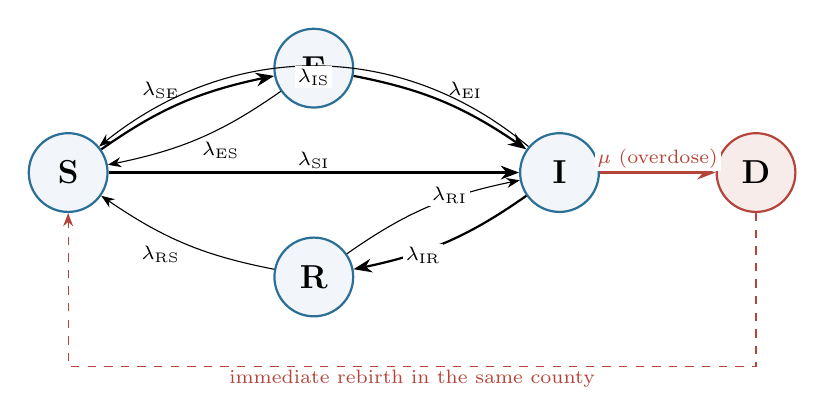
\begin{tikzpicture}[scale=0.78,>=Stealth,every node/.style={font=\small},
   cls/.style={circle,draw=accent,fill=soft,thick,minimum size=1.0cm,inner sep=1pt,font=\large\bfseries},
   lab/.style={font=\scriptsize,fill=white,inner sep=1pt}]
  \node[cls] (S) at (0,0) {S};
  \node[cls] (E) at (4,1.7) {E};
  \node[cls] (I) at (8,0) {I};
  \node[cls] (R) at (4,-1.7) {R};
  \node[cls,draw=tiedc,fill=tiedc!10] (D) at (11.2,0) {D};
  \draw[->,thick] (S) to[bend left=12] node[lab,above left] {$\lambda_{\Sc\Ec}$} (E);
  \draw[->] (E) to[bend left=12] node[lab,below right] {$\lambda_{\Ec\Sc}$} (S);
  \draw[->,thick] (E) to[bend left=12] node[lab,above right] {$\lambda_{\Ec\Ic}$} (I);
  \draw[->,thick] (S) -- node[lab,above] {$\lambda_{\Sc\Ic}$} (I);
  \draw[->,thick] (I) to[bend left=12] node[lab,below left] {$\lambda_{\Ic\Rc}$} (R);
  \draw[->] (R) to[bend left=12] node[lab,above right] {$\lambda_{\Rc\Ic}$} (I);
  \draw[->] (R) to[bend left=12] node[lab,below left] {$\lambda_{\Rc\Sc}$} (S);
  \draw[->] (I) to[bend right=40] node[lab,below] {$\lambda_{\Ic\Sc}$} (S);
  \draw[->,thick,tiedc] (I) -- node[lab,above] {$\mu$ (overdose)} (D);
  \draw[->,dashed,tiedc] (D.south) -- ++(0,-2.5) -| node[lab,pos=0.25,below] {immediate rebirth in the same county} (S.south);
 \end{tikzpicture}
 \vspace{-6pt}

 \begin{columns}[T]
 \column{0.48\textwidth}
 \begin{legend}
 \textbf{S} susceptible \quad \textbf{E} exposed: misusing opioids \quad \textbf{I} opioid use disorder (OUD) \quad \textbf{R} in treatment/recovery \quad \textbf{D} overdose death
 \end{legend}
 \column{0.48\textwidth}
 \begin{tied}
 $\Dc$ is a \emph{flux}, not a state: a dead agent is reborn as $\Sc$ at once. Population is closed, $s+e+i+r=1$, so the state is $3$-dimensional, $s=1-e-i-r$ is never an unknown.
 \end{tied}
 \end{columns}
\end{frame}

\begin{frame}{Dynamics: competing exponential clocks}
 Agent $i$ in class $X$ has out-rates $\lambda_{XY}(i,t)$ (per year). Let $\Lambda_X=\sum_Y\lambda_{XY}$. In one step $\Delta t$:
 \[
 \Pr\big(\text{leave}\big)=1-e^{-\Lambda_X\Delta t},\qquad
 \Pr\big(\text{destination }Y\mid\text{leave}\big)=\frac{\lambda_{XY}}{\Lambda_X}.
 \]
 \begin{columns}[T]
 \column{0.5\textwidth}
 \begin{block}{Why this form}\small
  It is the exact one-step law of a continuous-time Markov chain with generator $Q_{XY}=\lambda_{XY}$, $Q_{XX}=-\Lambda_X$, \emph{if the rates are frozen} over $\Delta t$.
  \begin{itemize}\setlength\itemsep{1pt}
   \item no $O(\Delta t)$ bias from ``$p=\lambda\Delta t$'': probabilities never exceed 1
   \item destinations are chosen \emph{proportionally}, so adding a competing exit never distorts the others' relative odds
  \end{itemize}
 \end{block}
 \column{0.47\textwidth}
 \begin{block}{What makes it non-trivial}\small
  The rates depend on the \emph{configuration}: neighbours' classes $\pi$ and market state $v,\varphi$. The process is therefore a nonlinear (McKean--Vlasov type) Markov process on $\{\Sc,\Ec,\Ic,\Rc\}^N$.
  \par\smallskip
  As $N\to\infty$ the expected shares are governed by an ODE (Section 6). This is the standard law-of-large-numbers heuristic; we do not prove it here, we \emph{check} it: noise shrinks by $\sqrt5$ when $N$ grows $5\times$.
 \end{block}
 \end{columns}
 \begin{kept}
  Weekly updates are synchronous (all agents read the same $(\pi,v,\varphi)$, then all draw): an Euler-type splitting with $O(\Delta t)$ error.
 \end{kept}
\end{frame}

%==================================================================
\section{2 Environment}
\begin{frame}{Raw variables $x$: what is observed}
 \footnotesize
 \renewcommand{\arraystretch}{1.08}
 \begin{tabular}{@{}l p{6.6cm} l p{4.2cm}@{}}
 \toprule
 Symbol & Variable & Unit & Years / source\\\midrule
 $x^{pov}$ & persons below poverty line & \% & 2012--23, ACS 5-yr\\
 $x^{unemp}$ & unemployment rate & \% & ACS\\
 $x^{inc}$ & median household income & USD & ACS\\
 $x^{nohs}$, $x^{bach}$ & adults 25+ without diploma; with bachelor's or more & \% & ACS\\
 $x^{dis}$, $x^{vet}$ & population with disability; adult veterans & \% & ACS\\
 $x^{unins}$ & without health insurance & \% & ACS\\
 $x^{age}$ & median age & years & ACS\\
 $x^{Rx}$ & opioid prescriptions per 100 residents & Rx/100 & CDC: county 2010--18, then national trend\\
 $x^{str}_s(t)$ & COVID policy stringency, per \emph{state} & 0--100 & OxCGRT, 2020--22\\
 $P_c$, tracts & county population; 33{,}696 tracts (centroid, area, pop.) & people & SRDDRC; Census 2020 + Gazetteer\\
 $Y_c(y)$ & \textbf{observed} overdose deaths (counts 1--9 hidden by CDC) & count & SRDDRC / CDC WONDER, 2010--23\\
 \bottomrule
 \end{tabular}
 \vspace{4pt}
 \begin{block}{Conventions}\small
  2010--11 have no county ACS: they reuse 2012. After the last data year every input is held at its last value; stringency is $0$ after 2022. Annual values are placed at mid-year and \emph{linearly interpolated} in $t$.
 \end{block}
\end{frame}


\begin{frame}{Worked example 1/2: standardising one county-year}
 \textbf{Case:} Barbour County, Alabama, 2019. Pooled means and SDs are over all $1538\times12$ county-years. For one variable the recipe is $z=(x-\bar x)/s_x$, then clip to $[-3,3]$.
 \par\smallskip
 \footnotesize\renewcommand{\arraystretch}{1.12}
 \begin{tabular}{@{}l r r r r l@{}}
 \toprule variable & $x$ (this county) & pooled mean $\bar x$ & SD $s_x$ & $z$ & reading\\\midrule
 poverty \% & 30.67 & 18.22 & 6.49 & $+1.92$ & much poorer than typical\\
 unemployment \% & 9.20 & 7.54 & 3.66 & $+0.45$ & slightly higher\\
 $\log$ median income & $\ln 32525=10.39$ & 10.71 & 0.264 & $-1.23$ & much lower income\\
 no diploma \% & 26.79 & 16.93 & 6.83 & $+1.44$ & \\
 bachelor's+ \% & 11.58 & 19.11 & 8.75 & $-0.86$ & \\
 disability \% & 21.38 & 17.25 & 4.57 & $+0.91$ & \\
 veterans \% & 6.62 & 9.22 & 3.00 & $-0.87$ & \\
 uninsured \% & 11.32 & 14.53 & 5.40 & $-0.59$ & \\
 median age & 40.4 & 40.34 & 5.01 & $+0.01$ & about average\\
 \bottomrule\end{tabular}
 \par\smallskip
 \begin{block}{How to read a $z$}\small
  $z=+1.92$ means ``1.92 standard deviations above the typical county-year''. Income is logged first because income gaps are ratios (a \$10k gap matters more at \$30k than at \$90k). The clip at $\pm3$ stops a single freak value (a tiny county) from dominating an index.
 \end{block}
\end{frame}

\begin{frame}{From variables to four indices $\xi$}
 \textbf{Step 1: standardise, pooled over all counties and years} (so real time trends survive):
 \[
  z^j_c(y)=\clip\!\Big(\frac{x^j_c(y)-\bar x^j}{s_j},\,-3,\,3\Big),\qquad j\in\{pov,unemp,nohs,bach,dis,vet,unins,age,\log inc\}.
 \]
 \textbf{Step 2: average within a theme, then re-standardise} ($\operatorname{std}$ = subtract mean, divide by SD):
 \begin{align*}
  \xi^{econ}&=\operatorname{std}\tfrac15\big(z^{pov}+z^{unemp}+z^{nohs}-z^{\log inc}-z^{bach}\big) &&\text{economic precarity}\\
  \xi^{pain}&=\operatorname{std}\tfrac12\big(z^{dis}+z^{vet}\big) &&\text{pain and injury burden}\\
  \xi^{unins}&=z^{unins},\qquad \xi^{age}=z^{age} &&\text{treatment barrier; older population}
 \end{align*}
 \begin{columns}[T]
 \column{0.5\textwidth}
 \begin{tied}
  Nine census variables collapse to \textbf{four} coordinates. $\xi^{unins},\xi^{age}$ are just $z$ (a one-variable index needs no new symbol; re-standardisation after clipping changes it negligibly).
 \end{tied}
 \column{0.47\textwidth}
 \begin{kept}
  \emph{Re-standardising} is not cosmetic: averaging shrinks variance, so without it ``one unit of $\xi^{econ}$'' would mean less than ``one unit of $\xi^{pain}$''. After it, \textbf{``per SD''} means the same thing for every index, and $\xi=0$ is the average county.
 \end{kept}
 \end{columns}
\end{frame}


\begin{frame}{Worked example 2/2: from nine $z$'s to four $\xi$'s}
 Same county. Signs: poverty, unemployment, no-diploma push \emph{up} precarity; income and bachelor's push it \emph{down}, hence the minus signs.
 \begin{align*}
  \text{raw econ}&=\tfrac15\big(1.92+0.45+1.44-(-1.23)-(-0.86)\big)=\tfrac{5.90}{5}=1.18\\
  \xi^{econ}&=\frac{1.18-\text{mean}}{\text{SD of raw econ}}=\frac{1.18-0}{0.795}=\mathbf{1.49}\\
  \xi^{pain}&=\operatorname{std}\tfrac12(0.91+(-0.87))=\operatorname{std}(0.02)=\mathbf{0.04},\qquad
  \xi^{unins}=\mathbf{-0.59},\quad \xi^{age}=\mathbf{0.01}
 \end{align*}
 \begin{columns}[T]
 \column{0.5\textwidth}
 \begin{block}{Why divide by 0.795?}\small
  Averaging five partly independent $z$'s makes the result vary less than a single $z$ (its SD is only $0.795$, not $1$). Dividing restores SD $=1$, so ``$\xi^{econ}=1.49$'' really means ``1.49 SD above average''. Check in the data: each $\xi^{econ},\xi^{pain}$ has mean $0$ and SD $1.00$ over all county-years.
 \end{block}
 \column{0.47\textwidth}
 \begin{block}{Reading the result}\small
  Barbour is \textbf{economically precarious} ($+1.5$ SD), has \textbf{average pain burden}, \textbf{slightly better insurance} than average, and \textbf{average age}. These four numbers are all the model ever knows about this county's census side.
 \end{block}
 \end{columns}
\end{frame}

\begin{frame}{The rate modifier $F$: a log-linear (proportional-hazards) link}
 Every rate $\theta\in\{\beta,\gamma,\sigma,\epsilon,\zeta,\nu,\mu,\delta,\rho\}$ in county $c$ is multiplied by
 \[
  F_\theta(c,t)=\exp\Big(\sum_{k\in\{econ,pain,unins,age\}} w_{\theta k}\,\xi^k_c(t)\Big)
  \qquad\Longleftrightarrow\qquad \log F_\theta = \bm w_\theta\cdot\bm\xi .
 \]
 \begin{columns}[T]
 \column{0.48\textwidth}
 \begin{kept}
  The exponential is not decoration:
  \begin{itemize}\setlength\itemsep{1pt}
   \item rates stay positive for any $\xi$;
   \item effects \emph{multiply} (a hazard-ratio, as in Cox regression);
   \item $w_{\theta k}$ is directly ``percent change in the rate per SD'';
   \item $\xi=0\Rightarrow F=1$: the average county keeps the literature baseline.
  \end{itemize}
 \end{kept}
 \column{0.5\textwidth}
 \begin{tied}
  A $4\times 9$ weight matrix looks like 36 parameters. It is not. We fix \emph{signs and relative mix} from the literature, $\bar w_{\theta k}$, and keep one scalar per index:
  \[ w_{\theta k}=s_k\,\bar w_{\theta k}. \]
  \textbf{Four free scalars}, $s_{econ},s_{pain},s_{unins},s_{age}$; the next slide pins them down.
 \end{tied}
 \end{columns}
\end{frame}


\begin{frame}{Worked example: turning $\xi$ into rate multipliers $F$}
 Weights from the table (per SD). For $\Ic\to\Dc$ ($\mu$), $\Ec\to\Ic$ ($\sigma$) and $\Sc\to\Ec$ ($\beta$) in Barbour ($\xi=(1.49,\,0.04,\,-0.59,\,0.01)$):
 \begin{align*}
  \log F_\beta&=0.0156(1.49)+(-0.10)(0.01)=0.0220 &&\Rightarrow F_\beta=e^{0.0220}=1.022\\
  \log F_\sigma&=0.0156(1.49)=0.0232 &&\Rightarrow F_\sigma=1.023\\
  \log F_\gamma&=0.2135(0.04)+0.20(0.01)=0.0103 &&\Rightarrow F_\gamma=1.010\\
  \log F_\mu&=0.0326(-0.59)+0.10(0.01)=-0.0182 &&\Rightarrow F_\mu=0.982
 \end{align*}
 \begin{columns}[T]
 \column{0.5\textwidth}
 \begin{block}{Reading}\small
  Each factor is within about $\pm2\%$ of 1. A county $1.5$ SD more precarious than average has misuse start $2\%$ faster, progress $2\%$ faster, and (thanks to better-than-average insurance) overdose $2\%$ \emph{slower}. Small per-rate shifts, but they compound through the feedback loop.
 \end{block}
 \column{0.47\textwidth}
 \begin{block}{Check yourself}\small
  Rule: $e^{x}\approx1+x$ for small $x$. So $F\approx1+\sum_kw_{\theta k}\xi^k$: read the weight as ``percent change in the rate per SD''. $0.0156\to1.6\%$ per SD of econ on $\beta$.
 \end{block}
 \end{columns}
\end{frame}

\begin{frame}{Elasticity matching: setting the four scalars $s_k$}
 Let $m^\ast(\bm\xi)$ be the long-run deaths per 10{,}000 of the averaged equations (Section 6) when county $\xi$ is perturbed. Choose $s_k$ so that
 \[
  \frac{\partial\ln m^\ast}{\partial\xi^k}\Big|_{\bm\xi=0}=\tau_k,\qquad
  (\tau_{econ},\tau_{pain},\tau_{unins})=(0.15,\,0.20,\,0.10),\quad s_{age}=1 .
 \]
 One-dimensional root finding (Brent) per index, using a symmetric difference with step $0.25$.
 \begin{columns}[T]
 \column{0.56\textwidth}
 \begin{block}{Result (weights per SD)}\tiny
 \renewcommand{\arraystretch}{1.15}
 \begin{tabular}{@{}l@{\hspace{3pt}}*{8}{c@{\hspace{3pt}}}@{}}
 \toprule
 & $\beta$ & $\gamma$ & $\sigma$ & $\epsilon$ & $\zeta$ & $\mu$ & $\delta$ & $\rho$\\\midrule
 $econ$ & $+.016$ & & $+.016$ & $-.010$ & $-.010$ & & $-.010$ & $+.010$\\
 $pain$ & & $+.213$ & & & & & &\\
 $unins$ & & & & & $-.049$ & $+.033$ & &\\
 $age$ & $-.10$ & $+.20$ & & & & $+.10$ & &\\\bottomrule
 \end{tabular}
 \par\smallskip
 Scale factors $s_k\approx 0.11,\ 0.71,\ 0.33,\ 1$ relative to the priors.
 \end{block}
 \column{0.41\textwidth}
 \begin{block}{Targets and why}\scriptsize
  $\tau_{econ}=15\%$/SD: unemployment alone gives about $6\%$ (Hollingsworth); Ruhm finds the economic channel smaller than the drug environment. $\tau_{pain}=20\%$: prescription exposure. $\tau_{unins}=10\%$: small, as the regional correlation is negative.
 \end{block}
 \end{columns}
 \begin{kept}
  Needed because the average county sits near the epidemic threshold ($\Rzero=0.79$): unscaled priors implied $\times4.5$ deaths per SD of econ and put $26\%$ of people in self-sustaining counties (runaway Texas). After matching: $4\%$.
 \end{kept}
\end{frame}

%==================================================================

\begin{frame}{Worked example: finding the scale $s_k$ numerically}
 \textbf{Question.} By what factor $s$ should the literature's weight pattern for econ be multiplied so that $+1$ SD gives $+15\%$ deaths?
 \par\smallskip
 \textbf{Step 1: compute $m^\ast$.} Solve the averaged equations (Section 6) to equilibrium with $F_\theta=\exp(s\,\bar w_{\theta,econ}\,x)$ at $x=-0.25,0,+0.25$:
 \par\smallskip
 \centering\footnotesize\renewcommand{\arraystretch}{1.15}
 \begin{tabular}{l ccc c}
 \toprule & $m^\ast(-0.25)$ & $m^\ast(0)$ & $m^\ast(+0.25)$ & elasticity $\dfrac{\ln m^\ast(.25)-\ln m^\ast(-.25)}{0.5}$\\\midrule
 prior weights, $s=1$ & 0.562 & 0.762 & 1.188 & $1.495\ \Rightarrow\ e^{1.495}=\times4.46$ per SD\\
 matched, $s=0.104$ & 0.734 & 0.762 & 0.792 & $0.150\ \Rightarrow\ +15\%$ per SD\\\bottomrule
 \end{tabular}
 \par\smallskip\raggedright\normalsize
 \textbf{Step 2: root-find.} The elasticity grows with $s$, so $f(s)=\text{elasticity}(s)-0.15$ has one root; Brent's method on $[10^{-4},3]$ gives $s_{econ}=0.104$. Likewise $s_{pain}=0.71$, $s_{unins}=0.33$.
 \begin{kept}
  Units: $m^\ast$ is deaths per 10{,}000 people per year. Age is untouched ($s=1$) and ends at elasticity $-0.037$ ($-3.7\%$ per SD).
 \end{kept}
\end{frame}

\section{3 Drug availability}
\begin{frame}{Three availability variables}
 \begin{tabularx}{\textwidth}{@{}l X X l@{}}
 \toprule
 Symbol & What & Law & Feeds\\\midrule
 $a_c(t)$ & prescription supply, Rx per person-year & $x^{Rx}_c/100$, interpolated in $t$ & $\Sc\to\Ic$\\[3pt]
 $v_c(t)$ & illicit supply index, $1$ = level at start & SDE driven by local demand (next slide) & $\Sc\to\Ec,\ \Ec\to\Ic,\ \Rc\to\Ic$\\[3pt]
 $\varphi_s(t)$ & fentanyl share of the illicit supply, state $s$ & Bass ODE with COVID forcing & $\Ic\to\Dc$\\
 \bottomrule
 \end{tabularx}
 \vspace{6pt}
 \begin{block}{Design choice: availability is dynamic and endogenous}\small
  Prescriptions $a$ are exogenous data. The illicit market is \emph{not}: it responds to the number of users ($v$), and its composition drifts toward fentanyl ($\varphi$). This feedback is what a fixed-coefficient regression cannot represent.
 \end{block}
 \begin{kept}
  Three separate variables rather than one ``availability'' scalar, because each acts on a different transition, with a different mechanism (onset by prescription, recruitment/relapse by supply, lethality by potency).
 \end{kept}
\end{frame}


\begin{frame}{Worked example: prescriptions $a$ and mid-year interpolation}
 \textbf{Raw:} Barbour County, 2019: $78.3$ prescriptions per 100 residents, so
 \[ a_c=\frac{x^{Rx}_c}{100}=\frac{78.3}{100}=0.783\ \text{prescriptions per person per year.}\]
 \textbf{Interpolating in time.} A yearly number describes the \emph{whole} year, so we pin it to mid-year, $t=y+\tfrac12$, and draw straight lines between neighbours:
 \[
  a(t)=(1-f)\,a(y)+f\,a(y+1),\qquad f=t-(y+\tfrac12).
 \]
 At $t=2019.25$ (end of March): $y=2018$ (anchor $2018.5$), $f=2019.25-2018.5=0.75$, so $a=0.25\,a(2018)+0.75\,a(2019)$.
 \begin{kept}
  The same interpolation is applied to every $\xi$, so rates change smoothly week by week instead of jumping on 1 January. Outside the data range the value is frozen at the first/last year (``flat'' extrapolation); this is what the 2060 projection assumes.
 \end{kept}
\end{frame}

\begin{frame}{Illicit supply $v$: a mean-reverting, spatially coupled SDE}
 \[
  \dd v_c=\Big[\kappa_v\big(v^\ast_c-v_c\big)+D_v\sum_{c'}W_{cc'}\big(v_{c'}-v_c\big)\Big]\dd t+\tau_v\,v_c\,\dd B_c,
  \qquad v_c(0)=1
 \]
 \[
  v^\ast_c=\Big(\frac{\mathcal D_c}{\bar{\mathcal D}_0}\Big)^{\theta_d},\quad
  \mathcal D_c=\operatorname{shrink}\!\big(i_c+\vartheta\,e_c\big),\quad
  W_{cc'}=\frac{e^{-d_{cc'}/\ell}}{\sum_{c''\ne c}e^{-d_{cc''}/\ell}}.
 \]
 \begin{columns}[T]
 \column{0.56\textwidth}
 \begin{legend}
 \begin{tabular}{@{}p{1.2cm}p{5.6cm}@{}}
 $\mathcal D_c$ & local demand: OUD share plus $\vartheta$ times misuse share\\
 $\bar{\mathcal D}_0$ & population-weighted regional demand when the run starts\\
 $\theta_d=0.1$ & demand elasticity of supply\\
 $\kappa_v=1$ & speed of adjustment (about one year)\\
 $D_v=0.2$ & spill-over strength; $\ell=100$ km\\
 $\tau_v=0.1$ & market volatility\\
 $d_{cc'}$ & distance between county centroids\\
 $B_c$ & independent Brownian motions
 \end{tabular}
 \end{legend}
 \column{0.41\textwidth}
 \begin{tied}
  $W$ is row-stochastic, so the coupling is $-D_v(I-W)v$: a random-walk graph Laplacian. One spill-over parameter and one length, not a matrix of weights. $\bar{\mathcal D}_0$ normalises the baseline to $v^\ast=1$.
 \end{tied}
 \begin{kept}
  Noise is \emph{multiplicative} ($\tau_v v\,\dd B$): a price-like index stays positive and fluctuates in relative terms.
 \end{kept}
 \end{columns}
\end{frame}


\begin{frame}{Worked example: one Euler step of the supply SDE}
 One county, $v_c=1.00$. Local demand is $20\%$ above baseline, neighbours average $\bar v_{nb}=\sum_{c'}W_{cc'}v_{c'}=1.05$. One week, $\Delta t=1/52$.
 \begin{align*}
  v^\ast&=(1.2)^{0.1}=1.018 &&\text{(target: 20\% more demand $\to$ only 1.8\% more supply, since $\theta_d=0.1$)}\\
  \text{drift}&=\kappa_v(1.018-1.00)+D_v(1.05-1.00)=0.018+0.010=0.028 &&\text{per year}\\
  \text{noise}&=\tau_v\,v\sqrt{\Delta t}\,Z=0.1\cdot1\cdot0.139\,Z=0.0139\,Z,\ Z\sim\mathcal N(0,1)\\
  v^{new}&=1.00+0.028\cdot\tfrac1{52}+0.0139Z=1.0005+0.0139Z
 \end{align*}
 \begin{columns}[T]
 \column{0.5\textwidth}
 \begin{block}{Reading}\small
  The deterministic pull per week ($+0.0005$) is much smaller than the random wobble ($\pm0.014$): the market is noisy week to week but is pulled back over about $1/\kappa_v=1$ year. The $\sqrt{\Delta t}$ is the Brownian scaling: noise variance grows linearly in time.
 \end{block}
 \column{0.47\textwidth}
 \begin{block}{Shrinking demand for a small county}\small
  $n_c=300$ agents, county demand $0.012$, regional $0.0066$, $k_0=20$:
  \[\mathcal D=\frac{300\cdot0.012+20\cdot0.0066}{320}=0.0117.\]
  Mostly the county's own value, nudged $3\%$ toward the region because 300 agents are few.
 \end{block}
 \end{columns}
\end{frame}

\begin{frame}{Fentanyl share $\varphi$: Bass diffusion with COVID forcing}
 \[
  \frac{\dd\varphi_s}{\dd t}=\big(p_{\mathrm{eff},s}(t)+q_\varphi\,\varphi_s\big)(1-\varphi_s),\qquad
  p_{\mathrm{eff},s}(t)=p_\varphi+p_{cov}\,\psi_s(t),\qquad \varphi_s=0\ \text{before }2013 .
 \]
 \begin{columns}[T]
 \column{0.5\textwidth}
 \begin{legend}
 \begin{tabular}{@{}p{1.0cm}p{6.2cm}@{}}
 $p_\varphi$ & spontaneous introduction (\emph{innovation}); fitted $0.0128$\\
 $q_\varphi$ & copying from markets that already switched (\emph{imitation}); assumed $0.6$\\
 $\psi_s(t)$ & stringency $\in[0,1]$, $=x^{str}_s/100$\\
 $p_{cov}$ & extra introduction per unit stringency; fitted $1.33$
 \end{tabular}
 \end{legend}
 Without COVID, closed form with $\tau=t-2013$:
 \[
  \varphi(\tau)=\frac{1-e^{-(p_\varphi+q_\varphi)\tau}}{1+\frac{q_\varphi}{p_\varphi}e^{-(p_\varphi+q_\varphi)\tau}} .
 \]
 \column{0.47\textwidth}
 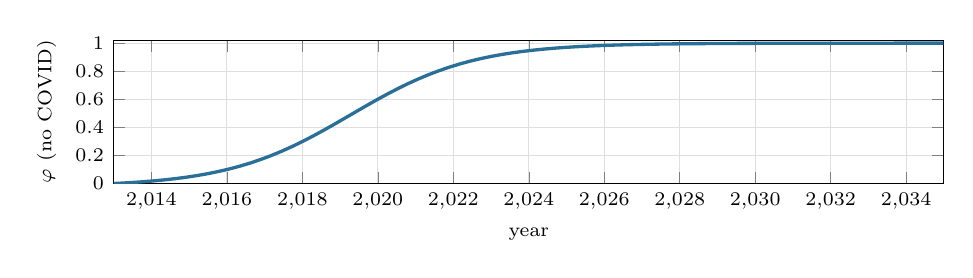
\begin{tikzpicture}
 \begin{axis}[width=\linewidth,height=3.4cm,xlabel={year},ylabel={$\varphi$ (no COVID)},xmin=2013,xmax=2035,ymin=0,ymax=1.02,
   tick label style={font=\scriptsize},label style={font=\scriptsize},grid=major,grid style={ink!15}]
 \addplot[accent,very thick,domain=2013:2035,samples=80]{(1-exp(-0.6128*(x-2013)))/(1+(0.6/0.0128)*exp(-0.6128*(x-2013)))};
 \end{axis}
 \end{tikzpicture}
 \par\vspace{-2pt}
 \begin{tied}
  $p_\varphi+p_{cov}\psi$ is one time-dependent innovation coefficient; COVID adds no new structure.
 \end{tied}
 \end{columns}
 \begin{kept}
  Two COVID effects are \emph{not} redundant: the push on $\varphi$ is \textbf{permanent} ($\varphi$ never falls when $\psi\to0$); the isolation effect $e^{w_{iso}\psi}$ is \textbf{temporary}. The data choose (Section 7).
 \end{kept}
\end{frame}

%==================================================================

\begin{frame}{Worked example: Bass curve for the fentanyl share}
 \textbf{Closed form, no COVID} ($p_\varphi=0.0128$, $q_\varphi=0.6$, year 2023 so $\tau=10$):
 \begin{align*}
  p_\varphi+q_\varphi&=0.6128,\qquad e^{-0.6128\cdot10}=e^{-6.128}=0.0022,\qquad q_\varphi/p_\varphi=46.9\\
  \varphi(2023)&=\frac{1-0.0022}{1+46.9\cdot0.0022}=\frac{0.9978}{1.1017}=\mathbf{0.906}
 \end{align*}
 \textbf{One weekly step with COVID} ($\varphi=0.20$, stringency $\psi=0.5$):
 \begin{align*}
  \frac{\dd\varphi}{\dd t}&=\big(0.0128+1.33\cdot0.5+0.6\cdot0.20\big)(1-0.20)=0.798\cdot0.80=0.638\ \text{per year}\\
  \varphi^{new}&=0.20+0.638/52=0.2123
 \end{align*}
 \begin{columns}[T]
 \column{0.5\textwidth}
 \begin{block}{Reading the three terms}\small
  $0.0128$: market is seeded spontaneously. $0.665$: pandemic supply disruption pushes it (the dominant term at $\psi=0.5$). $0.12$: copying, proportional to how far it already spread. $(1-\varphi)$: there is less market left to convert as $\varphi\to1$.
 \end{block}
 \column{0.47\textwidth}
 \begin{block}{Why it matters}\small
  $\varphi$ multiplies lethality: $\mu=\mu_H(1+2.88\varphi)$. Going $\varphi:0\to0.9$ makes overdose $\approx3.6\times$ deadlier. This one curve carries the entire rise of deaths in the model.
 \end{block}
 \end{columns}
\end{frame}

\section{4 Space}
\begin{frame}{Agents on real population geometry}
 \begin{columns}[T]
 \column{0.52\textwidth}
 \textbf{Placement.} $n_c=\big\lfloor N P_c/\sum P\big\rfloor$ agents per county (remainder to largest fractional parts). Agent $i\in c$:
 \begin{align*}
 \Pr(\tau(i)=\tau)&=\frac{\mathrm{pop}_\tau}{\sum_{\tau'\in c}\mathrm{pop}_{\tau'}},\\
 \bm u_i&=\bm c_\tau+\sqrt{U}\,r_\tau\,(\cos\Theta,\sin\Theta),
 \end{align*}
 with $U\sim\mathcal U[0,1]$, $\Theta\sim\mathcal U[0,2\pi]$, $r_\tau=\sqrt{A_\tau/\pi}$.
 \par\smallskip
 So the agent density is a \emph{piecewise-constant approximation of true population density}, uniform inside the disc that has the tract's area.
 \column{0.45\textwidth}
 \begin{legend}
 \begin{tabular}{@{}p{1.1cm}p{5.2cm}@{}}
 $\mathrm{pop}_\tau$ & tract population (Census 2020)\\
 $\bm c_\tau,\ A_\tau$ & tract centroid (km), area (km$^2$)\\
 $\bm u_i$ & location of agent $i$ in a projected plane\\
 $h=15$ km & interaction radius (30 km in the scale test)
 \end{tabular}
 \end{legend}
 \begin{kept}
  No ``crowding factor'' multiplies contacts. A version with one was removed: big metros became self-sustaining. Dense places have more agents, but each agent sees the same \emph{share} of users.
 \end{kept}
 \end{columns}
\end{frame}


\begin{frame}{Worked example: placing agents}
 A county has two tracts, populations $4{,}000$ and $6{,}000$ (cumulative weights $0.4,\ 1.0$), and the second tract has area $20$ km$^2$.
 \begin{enumerate}\setlength\itemsep{3pt}
  \item Draw $u=0.55$. The first cumulative weight $\ge0.55$ is $1.0$, so the agent goes to tract 2. (Tract 2 is chosen with probability $0.6$, exactly its population share.)
  \item Disc radius $r_\tau=\sqrt{A_\tau/\pi}=\sqrt{20/3.14}=2.52$ km. Draw $U=0.25$: distance from centroid $=\sqrt U\,r_\tau=0.5\cdot2.52=1.26$ km; draw $\Theta=1.0$ rad.
  \item Position $=\bm c_\tau+1.26(\cos1.0,\sin1.0)=\bm c_\tau+(0.68,\,1.06)$ km.
 \end{enumerate}
 \begin{block}{Why $\sqrt U$?}\small
  Area grows as $r^2$, so for points to be \emph{uniform} over the disc, $P(\text{dist}\le d)=d^2/r_\tau^2$. Inverting gives $d=r_\tau\sqrt U$. Using $U$ directly would pile points near the centre.
 \end{block}
 \begin{block}{Scale}\small
  $N=300{,}000$ agents for about $135$ million people: one agent represents about $450$ people. A county of $100{,}000$ gets $\approx222$ agents.
 \end{block}
\end{frame}

\begin{frame}{Local shares $\pi$: a Bayesian pseudo-count estimator}
 For class $X\in\{\Ec,\Ic,\Rc\}$ and agent $i$ with $B_i=\{j\ne i:\|\bm u_j-\bm u_i\|\le h\}$:
 \[
  \pi^X_i=\frac{\#\{j\in B_i:X_j=X\}+k_0\,x_{c(i)}}{|B_i|+k_0},\qquad k_0=20,
  \qquad x_c=\text{county fraction of class }X .
 \]
 \begin{columns}[T]
 \column{0.5\textwidth}
 \begin{kept}
  This is the posterior mean of a Beta--Binomial model with prior mean $x_c$ and prior strength $k_0$:
  \begin{itemize}\setlength\itemsep{1pt}
   \item $|B_i|\to\infty$: $\pi\to$ the empirical share, \emph{independent of $N$};
   \item $|B_i|=0$ (rural agent): $\pi=x_c$, no $0/0$;
   \item a lone neighbour cannot swing $\pi$ to $0$ or $1$.
  \end{itemize}
 \end{kept}
 \column{0.47\textwidth}
 \begin{tied}
  The \emph{same} shrinkage operator is reused for demand in $v^\ast$:
  \[ \operatorname{shrink}(d_c)=\frac{n_c\,d_c+k_0\,\bar d}{n_c+k_0},\]
  with $\bar d$ the regional average. One concept, one constant $k_0$.
 \end{tied}
 \end{columns}
 \begin{block}{Computation}\small
  Counts per class are binned on a $5$ km grid and convolved with the discretised disc $\{(a,b):(a^2+b^2)\,5^2\le h^2\}$. Cost is linear in $N$ plus grid size, instead of quadratic.
 \end{block}
\end{frame}

%==================================================================

\begin{frame}{Worked example: computing a local share $\pi$}
 $k_0=20$ pseudo-agents sit at the county's average. County fraction of OUD $i_c=0.006$.
 \par\smallskip
 \small\renewcommand{\arraystretch}{1.2}
 \begin{tabular}{@{}l c c l@{}}
 \toprule Agent's surroundings & neighbours $|B_i|$ & of which $\Ic$ & $\pi^I_i=\dfrac{\#\Ic+20(0.006)}{|B_i|+20}$\\\midrule
 city centre & 5000 & 30 & $\dfrac{30.12}{5020}=0.0060$\\[6pt]
 suburb & 12 & 1 & $\dfrac{1.12}{32}=0.035$\\[6pt]
 rural, nobody within 15 km & 0 & 0 & $\dfrac{0.12}{20}=0.006=i_c$\\\bottomrule
 \end{tabular}
 \par\smallskip
 \begin{columns}[T]
 \column{0.5\textwidth}
 \begin{block}{Reading}\small
  City: the data speak, $\pi\approx$ raw share $0.0060$. Suburb: one user among 12 neighbours would be $1/12=8.3\%$, which is too confident; the pseudo-agents pull it to $3.5\%$. Rural: no information, so use the county average.
 \end{block}
 \column{0.47\textwidth}
 \begin{block}{The $5$ km grid trick}\small
  Instead of testing all pairs, count each class per $5$ km cell, then sum counts over cells inside the disc. The disc kernel is all offsets $(a,b)$ with $a^2+b^2\le(15/5)^2=9$: a $7\times7$ block with the 4 corners removed gives \textbf{29 cells}. Cost $\propto N$.
 \end{block}
 \end{columns}
\end{frame}

\section{5 Rates}
\begin{frame}{Template: baseline $\times$ availability $\times$ modifier (+ peers)}
 \[
  \boxed{\ \lambda_{XY}(i,t)=\Big[\ \lambda^0_{XY}\cdot g_{XY}\big(a_c,v_c,\varphi_s,\psi_s\big)\ +\ \gamma_{XY}\,\pi^{Z}_i\ \Big]\cdot F_{XY}(c,t)\ }
 \]
 \begin{columns}[T]
 \column{0.48\textwidth}
 \begin{legend}
 \begin{tabular}{@{}p{1.2cm}p{5.8cm}@{}}
 $\lambda^0_{XY}$ & literature / calibrated baseline (per person-year)\\
 $g_{XY}$ & availability term; $\equiv1$ if the move does not depend on drug supply\\
 $\gamma_{XY}\pi^Z$ & peer term, only where the mechanism is social\\
 $F_{XY}$ & modifier $\exp(\bm w\cdot\bm\xi)$; $\equiv1$ where no index acts
 \end{tabular}
 \end{legend}
 \column{0.5\textwidth}
 \begin{tied}
  Nine rates, \emph{one} template. Each rate is read as the answer to three questions: what is the base speed, what does the drug market add, and who is nearby. A rate with no entry in a slot has that slot set to $1$ (or $0$ for peers).
 \end{tied}
 \begin{kept}
  This is the ``every rate = baseline $\times f$(environment)'' principle: no rate is a free constant.
 \end{kept}
 \end{columns}
 \vspace{2pt}
 \begin{block}{Two shared pieces defined once}\scriptsize
 \[
  \Pi_i=\pi^I_i+\vartheta\,\pi^E_i\quad(\text{contagion pressure; $\vartheta=0.3$: a misuser recruits less than a user}),\qquad
  \alpha=\gamma_{Rx}\,\chi .
 \]
 \end{block}
\end{frame}

\begin{frame}{The nine rates (per person-year)}
 \renewcommand{\arraystretch}{1.28}
 \footnotesize
 \begin{tabularx}{\textwidth}{@{}c l X@{}}
 \toprule
 & Rate $\lambda$ & Mechanism\\\midrule
 $\Sc\!\to\!\Ec$ & $\beta^0\,\Pi_i\,v_c\,F_\beta$ & misuse starts through nearby users; easier when supply is high\\
 $\Sc\!\to\!\Ic$ & $\alpha\,a_c\,F_\gamma$ & addiction onset from a prescription\\
 $\Ec\!\to\!\Ic$ & $\sigma^0\,v_c^{1/2}\,F_\sigma$ & misuse progresses to OUD\\
 $\Ec\!\to\!\Sc$ & $\epsilon^0\,F_\epsilon$ & misuser stops\\
 $\Ic\!\to\!\Rc$ & $\zeta^0F_\zeta+\gamma_p\,\pi^R_i$ & enters treatment; peers in recovery help\\
 $\Ic\!\to\!\Sc$ & $\nu^0$ & quits without treatment\\
 $\Ic\!\to\!\Dc$ & $\mu_H\big[1+\kappa\,\varphi_s\big]\,e^{w_{iso}\psi_s}\,F_\mu$ & overdose; $\kappa=m_F-1$ is the excess lethality of fentanyl\\
 $\Rc\!\to\!\Sc$ & $\delta^0F_\delta$ & lasting recovery\\
 $\Rc\!\to\!\Ic$ & $\big(\rho^0v_c^{1/2}+\rho_p\,\pi^I_i\big)F_\rho$ & relapse: from supply and from users nearby\\
 \bottomrule
 \end{tabularx}
 \vspace{4pt}
 \begin{tied}
  (i) $(1-\varphi)\mu_H+m_F\mu_H\varphi=\mu_H(1+\kappa\varphi)$, so the lethality mix is one number $\kappa=m_F-1\approx2.88$, and $\varphi=0\Rightarrow\mu_H$ exactly.
  (ii) The three supply exponents were $1,\tfrac12,\tfrac12$: write $v$, $v^{1/2}$, $v^{1/2}$ directly.
  (iii) $\Ic\!\to\!\Sc$ carries no modifier (none acts), so no empty $F_\nu$.
 \end{tied}
\end{frame}


\begin{frame}{Worked example: one weekly draw for two agents}
 \small Barbour agents: $\alpha=2.25\times10^{-4}$, $a=0.783$, $v=1.2$, $\varphi=0.5$, $\psi=0.5$, $\kappa=2.88$, $w_{iso}=0.14$, and the $F$'s from before.
 \par\smallskip
 \begin{columns}[T]
 \column{0.5\textwidth}
 \begin{block}{Agent in $\Sc$ ($\pi^I=\pi^E=0.008$)}\footnotesize
 \begin{align*}
  \Pi&=0.008+0.3(0.008)=0.0104\\
  \lambda_{\Sc\Ec}&=0.841\cdot0.0104\cdot1.2\cdot1.022=0.0107\\
  \lambda_{\Sc\Ic}&=2.25{\times}10^{-4}\cdot0.783\cdot1.010=0.00018\\
  \Lambda&=0.0109\\
  \Pr(\text{leave})&=1-e^{-0.0109/52}=0.00021\\
  \Pr(\to\Ec\mid\text{leave})&=0.0107/0.0109=98.4\%
 \end{align*}
 \end{block}
 \column{0.5\textwidth}
 \begin{block}{Agent in $\Ic$ ($\pi^R=0.004$)}\footnotesize
 \begin{align*}
  \lambda_{\Ic\Dc}&=0.0127(1+2.88\cdot0.5)\,e^{0.14\cdot0.5}\cdot0.982=0.0326\\
  \lambda_{\Ic\Rc}&=0.5(1.014)+0.1(0.004)=0.507\\
  \lambda_{\Ic\Sc}&=0.05\\
  \Lambda&=0.590\\
  \Pr(\text{leave})&=1-e^{-0.590/52}=0.0113\\
  \Pr(\Rc,\Sc,\Dc\mid\text{leave})&=86.0\%,\ 8.5\%,\ 5.5\%
 \end{align*}
 \end{block}
 \end{columns}
 \begin{block}{Reading}\small
  Almost no susceptible agent changes class in a given week ($0.02\%$), and when one does it nearly always becomes a misuser. An OUD agent leaves with probability about $1.1\%$ per week ($\approx45\%$ per year); $5.5\%$ of leavers die. The agent actually moves if a uniform $u_1<0.0113$; then $u_2\cdot\Lambda$ is compared with the cumulative rates $(0.507,\,0.557,\,0.590)$ to pick the destination.
 \end{block}
\end{frame}

\begin{frame}{Where redundancy was kept, and why}
 \small
 \begin{columns}[T]
 \column{0.5\textwidth}
 \begin{kept}
  \textbf{$\alpha=\gamma_{Rx}\chi$ is split.} Only the product is identifiable, but each factor has its own \emph{source}: $\gamma_{Rx}=0.0074$ (onset per therapy-year, literature) and $\chi\approx0.03$ (share on therapy per Rx per capita, calibrated). Keeping both lets a reader check each against a different paper.
 \end{kept}
 \begin{kept}
  \textbf{$\sigma^0$ and $\epsilon^0$ are both kept} although $\sigma^0+\epsilon^0=1$. Reparametrise as time $T_E=1/(\sigma^0+\epsilon^0)=1$ yr and progression probability $p=\sigma^0/(\sigma^0+\epsilon^0)=0.08$. The modifiers $F_\sigma\neq F_\epsilon$ act on the two separately, so the sum is not conserved.
 \end{kept}
 \column{0.47\textwidth}
 \begin{kept}
  \textbf{Peer terms next to baselines} ($\gamma_p\pi^R$, $\rho_p\pi^I$). The baseline alone gives a well-mixed ODE; the peer term is the only place space enters the rates besides $\beta$. Dropping it would delete the model's spatial content.
 \end{kept}
 \begin{kept}
  \textbf{$\vartheta$ appears twice} (in $\Pi$ and in demand $\mathcal D$). It is deliberately one symbol: whoever recruits also draws supply.
 \end{kept}
 \begin{kept}
  \textbf{Bass $p$ and $q$.} Innovation and imitation are different mechanisms (external vs.\ contagious), so two parameters.
 \end{kept}
 \end{columns}
\end{frame}

\begin{frame}{Parameters: value, status, basis}
 \scriptsize
 L = literature, A = assumption, C = calibrated to a \emph{non-death} target, F = fitted to deaths.
 \par\vspace{3pt}
 \renewcommand{\arraystretch}{1.12}
 \begin{tabularx}{\textwidth}{@{}l l c X@{}}
 \toprule
 Symbol & Value & St. & Basis\\\midrule
 $\beta^0$ & $0.841$ & C & new misuse $=0.66\%$ of people per year\\
 $\alpha=\gamma_{Rx}\chi$ & $0.0074\times0.03$ & L$\cdot$C & onset per therapy year [Battista]; $\chi\approx0.03$ chosen so OUD prevalence $=0.6\%$\\
 $\sigma^0,\epsilon^0$ & $0.08,\ 0.92$ & A & about one year of misuse; $8\%$ progress\\
 $\zeta^0,\ \delta^0$ & $0.5,\ 0.1$ & L & treatment entry; successful treatment [Battista]\\
 $\rho^0,\ \rho_p$ & $0.7,\ 0.2$ & L & about $90\%$ relapse within a year\\
 $\nu^0,\ \gamma_p,\ \vartheta$ & $0.05,\ 0.1,\ 0.3$ & A & slow untreated remission; peer recovery; recruiting power of $\Ec$\\
 $\mu_H$ & $0.0127$ & L & $12.7$ deaths per 1{,}000 untreated person-years [Sordo]\\
 $m_F=1+\kappa$ & $3.88$ & F & fentanyl market makes overdose $3.9\times$ deadlier\\
 $p_\varphi,\ q_\varphi$ & $0.0128,\ 0.6$ & F, A & fentanyl introduction and copying\\
 $p_{cov},\ w_{iso}$ & $1.33,\ 0.14$ & F & COVID supply push; isolation effect ($\times1.07$ at $\psi=0.5$)\\
 $\theta_d,\kappa_v,D_v,\tau_v$ & $0.1,1,0.2,0.1$ & A & supply follows demand within about a year\\
 $h,\ k_0,\ \ell$ & $15$ km, $20$, $100$ km & A & interaction radius, pseudo-count, spill-over length\\
 $s_k$ & $0.11,0.71,0.33,1$ & C & elasticity matching (targets from literature)\\
 \bottomrule
 \end{tabularx}
\end{frame}

%==================================================================
\section{6 Analysis}
\begin{frame}{Averaged equations (well-mixed county)}
 Replace $\pi^X\to x$ (the class fractions) and drop space. With $s=1-e-i-r$ and $v,a,\varphi,\psi$ held fixed,
 \begin{align*}
  \dot e&=\lambda_{\Sc\Ec}\,s-(\lambda_{\Ec\Ic}+\lambda_{\Ec\Sc})\,e,\\
  \dot i&=\lambda_{\Sc\Ic}\,s+\lambda_{\Ec\Ic}\,e+\lambda_{\Rc\Ic}\,r-(\lambda_{\Ic\Rc}+\lambda_{\Ic\Sc}+\mu)\,i,\\
  \dot r&=\lambda_{\Ic\Rc}\,i-(\lambda_{\Rc\Sc}+\lambda_{\Rc\Ic})\,r,
 \end{align*}
 where $\lambda_{\Sc\Ec}=\beta^0(i+\vartheta e)vF_\beta$ and $\lambda_{\Ic\Rc}=\zeta^0F_\zeta+\gamma_p r$, $\lambda_{\Rc\Ic}=(\rho^0v^{1/2}+\rho_pi)F_\rho$.
 \begin{columns}[T]
 \column{0.5\textwidth}
 \begin{block}{Role}\small
  (a) calibration; (b) $m^\ast$ for elasticity matching; (c) $\Rzero$; (d) sanity check of the agent code (the agent mean converges to it as $N\to\infty$).
 \end{block}
 \column{0.47\textwidth}
 \begin{kept}
  \textbf{No drug-free endpoint.} If $a>0$ then $\lambda_{\Sc\Ic}>0$ keeps injecting cases, so $i^\ast>0$: use never fully disappears while prescriptions exist. This is a structural property, not a fitted result.
 \end{kept}
 \end{columns}
\end{frame}


\begin{frame}{Worked example: the averaged equations at the calibrated point}
 \textbf{Check that $\dot e=0$ at the calibrated state} $(s,e,i,r)=(0.9836,\ 0.0066,\ 0.0060,\ 0.0037)$, $F=1$, $v=1$:
 \begin{align*}
  \lambda_{\Sc\Ec}&=\beta^0(i+\vartheta e)=0.841\,(0.0060+0.3\cdot0.0066)=0.841\cdot0.00798=0.00671\\
  \text{inflow to E}&=\lambda_{\Sc\Ec}\,s=0.00671\cdot0.9836=\mathbf{0.0066}\quad(\text{= target flux }f)\\
  \text{outflow from E}&=(\sigma^0+\epsilon^0)\,e=(0.08+0.92)(0.0066)=\mathbf{0.0066}\quad\Rightarrow\ \dot e=0\ \checkmark
 \end{align*}
 \begin{columns}[T]
 \column{0.5\textwidth}
 \begin{block}{Meaning of each equation}\small
  $\dot e$: new misusers arriving from $\Sc$ minus those who progress or quit. $\dot i$: arrivals from $\Sc$ (prescription), from $\Ec$ (progression), from $\Rc$ (relapse) minus exits to treatment, remission, death. $\dot r$: arrivals from $\Ic$ minus exits to $\Sc$ or back to $\Ic$. Each term is ``rate $\times$ share of the class it leaves''.
 \end{block}
 \column{0.47\textwidth}
 \begin{block}{Death does not appear as a loss}\small
  The $\mu\,i$ term leaves $\Ic$ but is added to $\dot s$ (rebirth), so shares still sum to 1. Check: $\dot s+\dot e+\dot i+\dot r=0$.
 \end{block}
 \end{columns}
\end{frame}

\begin{frame}{Closed-form calibration of $\beta^0$ and $\chi$}
 Targets at the reference point ($F=1$, $v=1$, $\varphi=0$, $\psi=0$, $a=\bar a$ the 2010 mean): prevalence $i^\ast=0.006$ and misuse flux $f=0.0066$ per year.
 Setting $\dot e=\dot i=\dot r=0$ gives, in order,
 \begin{align*}
  e^\ast&=\frac{f}{\sigma^0+\epsilon^0},\qquad
  r^\ast=\frac{\zeta^0\,i^\ast}{\rho^0+\delta^0+(\rho_p-\gamma_p)\,i^\ast},\qquad s^\ast=1-e^\ast-i^\ast-r^\ast,\\
  \beta^0&=\frac{f}{(i^\ast+\vartheta e^\ast)\,s^\ast},\qquad
  \alpha=\frac{(\zeta^0+\gamma_pr^\ast+\nu^0+\mu_H)\,i^\ast-\sigma^0e^\ast-(\rho^0+\rho_pi^\ast)\,r^\ast}{\bar a\;s^\ast},\quad \chi=\alpha/\gamma_{Rx}.
 \end{align*}
 \begin{columns}[T]
 \column{0.52\textwidth}
 \begin{tied}
  Two unknowns, two linear-in-unknown equations: \textbf{no optimisation}. Of the roughly 25 symbols, $\beta^0$ and $\chi$ are not free; they are \emph{consequences} of the two prevalence/flux targets. Start fractions $(s,e,i,r)=(98.3,\,0.66,\,0.60,\,0.38)\%$.
 \end{tied}
 \column{0.45\textwidth}
 \begin{block}{Feasibility}\small
  Need $\alpha\ge0$: progression plus relapse inflow must not already exceed the target outflow of $\Ic$. This failed for $\sigma^0=0.15$, which is why $\sigma^0=0.08$.
 \end{block}
 \end{columns}
\end{frame}


\begin{frame}{Worked example: calibrating $\beta^0$ and $\alpha$ step by step}
 Inputs: $i^\ast=0.006$, $f=0.0066$, $\sigma^0=0.08$, $\epsilon^0=0.92$, $\zeta^0=0.5$, $\rho^0=0.7$, $\rho_p=0.2$, $\gamma_p=0.1$, $\delta^0=0.1$, $\nu^0=0.05$, $\mu_H=0.0127$, $\vartheta=0.3$, $\bar a\approx1.01$.
 \footnotesize
 \begin{align*}
  e^\ast&=\frac{0.0066}{0.08+0.92}=0.0066\\
  r^\ast&=\frac{0.5(0.006)}{0.7+0.1+(0.2-0.1)(0.006)}=\frac{0.003}{0.8006}=0.003747\\
  s^\ast&=1-0.0066-0.006-0.003747=0.983653\\
  \beta^0&=\frac{0.0066}{(0.006+0.3\cdot0.0066)\,0.983653}=\frac{0.0066}{0.007850}=\mathbf{0.841}\\
  \text{outflow of I}&=(0.5+0.1\cdot0.003747+0.05+0.0127)(0.006)=0.003378\\
  \text{inflow to I from E, R}&=0.08(0.0066)+(0.7+0.2\cdot0.006)(0.003747)=0.000528+0.002627=0.003155\\
  \alpha&=\frac{0.003378-0.003155}{1.01\cdot0.983653}=\frac{0.000223}{0.9935}=\mathbf{2.2\times10^{-4}}\ \ (\chi=\alpha/\gamma_{Rx}\approx0.03)
 \end{align*}
 \normalsize
 \textbf{Reading.} Prescription onset must fill exactly the small gap ($0.000223$ per year) between who leaves $\Ic$ and who comes back by progression and relapse. This gap is tiny because relapse already feeds $\Ic$ strongly.
\end{frame}

\begin{frame}{Contact reproduction number $\Rzero$}
 Expected secondary misusers produced by one misuser through \emph{contact alone} (peer terms and prescriptions off, $s\approx1$):
 \[
  \Rzero=\beta^0\Big[\underbrace{\frac{\vartheta}{\sigma^0+\epsilon^0}}_{\text{while in }\Ec}+\frac{\sigma^0}{\sigma^0+\epsilon^0}\,T_I\Big],\qquad
  T_I=\frac{1}{\Lambda_I-\zeta^0\,\dfrac{\rho^0}{\rho^0+\delta^0}},\quad \Lambda_I=\zeta^0+\nu^0+\mu_H .
 \]
 \begin{columns}[T]
 \column{0.52\textwidth}
 \begin{block}{Derivation of $T_I$ (first-step analysis)}\scriptsize
  Let $T$ = expected total time in $\Ic$, counting relapses. From $\Ic$: stay $1/\Lambda_I$; with probability $\zeta^0/\Lambda_I$ go to $\Rc$, from which relapse (before $\Rc\to\Sc$) has probability $p_{RI}=\rho^0/(\rho^0+\delta^0)$:
  \[T=\tfrac1{\Lambda_I}+\tfrac{\zeta^0}{\Lambda_I}\,p_{RI}\,T\ \Rightarrow\ T_I=\frac{1}{\Lambda_I-\zeta^0p_{RI}}.\]
 \end{block}
 \column{0.45\textwidth}
 \begin{legend}
 $T_I\approx 7.99$ years in $\Ic$ per episode chain; $\Rzero=0.841\,[0.08\cdot7.99+0.3]=0.79$.
 \end{legend}
 \begin{kept}
  $\Rzero<1$ but close. A county whose modifiers lift $\Rzero$ by about $25\%$ becomes self-sustaining. This is the quantitative reason the weights $w$ must be sized by elasticity matching.
 \end{kept}
 \end{columns}
 \begin{block}{Tipping point in supply}\scriptsize
  If $\theta_d>0.2$ the supply--demand feedback destabilises the endemic state. We take $\theta_d=0.1$ (found numerically; a stability proof is open).
 \end{block}
\end{frame}

%==================================================================

\begin{frame}{Worked example: reading $\Rzero$}
 \small
 \begin{align*}
  \Lambda_I&=0.5+0.05+0.0127=0.5627,\qquad p_{RI}=\frac{0.7}{0.7+0.1}=0.875\\
  \zeta^0p_{RI}&=0.4375,\qquad T_I=\frac1{0.5627-0.4375}=\frac1{0.1252}=7.99\ \text{years}\\
  \Rzero&=0.841\Big[\underbrace{\tfrac{0.3}{1.0}}_{\text{misuse stage}}+\underbrace{\tfrac{0.08}{1.0}\cdot7.99}_{0.639}\Big]=0.841\cdot0.939=\mathbf{0.79}
 \end{align*}
 \begin{columns}[T]
 \column{0.5\textwidth}
 \begin{block}{Where the 8 years come from}\small
  One visit to $\Ic$ lasts $1/\Lambda_I=1.8$ years. A visit ends in treatment with probability $0.5/0.5627=0.89$, and $87.5\%$ of those relapse, so the chance of coming back is $0.78$. Expected visits $=1/(1-0.78)=4.5$, so $4.5\times1.8\approx8$ years in $\Ic$.
 \end{block}
 \column{0.47\textwidth}
 \begin{block}{Distance to threshold}\small
  $\Rzero=1$ needs a $1/0.79=1.27$ factor. A county has $F_\beta\approx F_\sigma\approx e^{0.016\,\xi^{econ}}$, so the weights alone move $\Rzero$ by only $\sim2\%$ per SD; unscaled priors moved it $\sim$10$\times$ more, which is why Texas ran away.
 \end{block}
 \end{columns}
\end{frame}

\section{7 Data link}
\begin{frame}{Expected deaths: a Rao--Blackwell estimator}
 Counting simulated deaths is noisy: a county of 300 agents holds about 2 OUD agents. Instead, accumulate the \emph{hazard}:
 \[
  \widehat m_c(y)=\frac{P_c(y)}{n_c}\sum_{k:\,t_k\in y}\Delta t\!\!\sum_{i:\,c(i)=c}\ind\{X_i(t_k)=\Ic\}\;\lambda_{\Ic\Dc}(i,t_k),\qquad
  \widehat M_s(y)=\sum_{c\in s}\widehat m_c(y).
 \]
 \begin{columns}[T]
 \column{0.5\textwidth}
 \begin{legend}
 \begin{tabular}{@{}p{1.3cm}p{5.6cm}@{}}
 $P_c/n_c$ & scale from agents to real people\\
 $\lambda_{\Ic\Dc}$ & overdose rate from the table\\
 $\widehat M_s$ & model expected deaths, state $s$, year $y$
 \end{tabular}
 \end{legend}
 \column{0.47\textwidth}
 \begin{kept}
  Same mean as counting deaths (the death indicator has conditional mean $\lambda\Delta t$), strictly smaller variance by the law of total variance. Conditioning on the path of classes removes the Bernoulli death noise.
 \end{kept}
 \end{columns}
\end{frame}


\begin{frame}{Worked example: expected deaths for one county-year}
 County with $P_c=100{,}000$ people, $n_c=222$ agents. Prevalence $0.6\%$, so on average $222\cdot0.006=1.33$ agents are in $\Ic$ at any time. Their overdose rate (as before) $\lambda_{\Ic\Dc}\approx0.033$ per year.
 \begin{align*}
  \sum_{k\in y}\Delta t\sum_i\ind\{X_i=\Ic\}\lambda_{\Ic\Dc}&\approx\underbrace{52}_{\text{weeks}}\cdot\tfrac1{52}\cdot1.33\cdot0.033=0.044\ \text{agent-deaths}\\
  \widehat m_c&=\frac{P_c}{n_c}\cdot0.044=450\cdot0.044=\mathbf{19.8}\ \text{real deaths}
 \end{align*}
 \begin{columns}[T]
 \column{0.5\textwidth}
 \begin{block}{Reading}\small
  Directly: $100{,}000\times0.6\%=600$ OUD people, times $0.033$ deaths/yr $=19.8$. The agent version gives the same answer with sample noise. Counting actual agent deaths would be 0 or 1 ($0.044$ expected), a hopeless signal; the hazard version contributes the smooth $0.044$ every week.
 \end{block}
 \column{0.47\textwidth}
 \begin{block}{State total}\small
  Sum $\widehat m_c$ over the counties of a state (e.g.\ $\approx1{,}900$ for a large state). Counties with no agents are removed from \emph{both} model and data so the comparison stays like-for-like.
 \end{block}
 \end{columns}
\end{frame}

\begin{frame}{Observation model: interval-censored negative binomial}
 CDC hides county counts of $1$--$9$. For state $s$, year $y$, the observed total lies in $[L_{sy},U_{sy}]$:
 \[
  L_{sy}=\sum_{c\in s}\big(Y^{\mathrm{vis}}_c+1\cdot\ind_{\mathrm{hid}}\big),\qquad
  U_{sy}=\sum_{c\in s}\big(Y^{\mathrm{vis}}_c+9\cdot\ind_{\mathrm{hid}}\big).
 \]
 Model total $\sim\mathrm{NB}(\text{mean }\widehat M_{sy},\text{size }r)$ with $\mathrm{Var}=\widehat M+\widehat M^2/r$, $r=50$:
 \[
  \ell_{sy}=\log\Big[\nbc\big(U_{sy};\,r,\tfrac{r}{r+\widehat M_{sy}}\big)-\nbc\big(L_{sy}-1;\,r,\tfrac{r}{r+\widehat M_{sy}}\big)\Big],\qquad
  \mathrm{score}=\frac1{|\mathcal S||\mathcal Y|}\sum_{s,y}\ell_{sy}.
 \]
 \begin{columns}[T]
 \column{0.5\textwidth}
 \begin{kept}
  \textbf{Why an interval, not a number.} Replacing a hidden count by 5 would fabricate precision and bias; the likelihood of the \emph{event} ``total in $[L,U]$'' is honest. \textbf{Why NB:} counts are over-dispersed relative to Poisson (CV $\approx1/\sqrt r=14\%$ for large means).
 \end{kept}
 \column{0.47\textwidth}
 \begin{tied}
  County-level scoring was \textbf{dropped}: at 300k agents the county signal is noise. The score lives at state level only, where $\widehat M$ is large.
 \end{tied}
 \end{columns}
\end{frame}


\begin{frame}{Worked example: scoring one state-year}
 A state-year has 12 suppressed counties and visible deaths $400$. Each hidden count is between $1$ and $9$:
 \[ L=400+12\cdot1=412,\qquad U=400+12\cdot9=508. \]
 Model mean $\widehat M$, $r=50$, success parameter $q=r/(r+\widehat M)$. Probability the model's total lands in $[412,508]$:
 \par\smallskip
 \centering\small\renewcommand{\arraystretch}{1.2}
 \begin{tabular}{c c c l}
 \toprule model mean $\widehat M$ & $\Pr(412\le Y\le508)$ & $\ell=\log\Pr$ & comment\\\midrule
 450 & 0.518 & $-0.66$ & model sits inside the interval\\
 600 & 0.139 & $-1.97$ & too high, but the spread is wide\\
 300 & 0.012 & $-4.40$ & too low, heavily penalised\\\bottomrule
 \end{tabular}
 \par\smallskip\raggedright
 \begin{block}{Reading the score}\small
  The overall score is the \emph{average} $\ell$ over all $17\times14$ state-years: $-2.44$ means on average the model gives about $e^{-2.44}\approx9\%$ probability to the observed interval. The earlier model scored $-70$ (probability essentially $0$). A perfect model would approach $0$.
 \end{block}
\end{frame}

\begin{frame}{Fitting four numbers without re-running agents}
 \[
  \bm\theta=(m_F,\ p_\varphi,\ p_{cov},\ w_{iso}),\qquad
  \lambda_{\Ic\Dc,s}(t;\bm\theta)=\mu_H\big[1+(m_F-1)\varphi_s(t;p_\varphi,p_{cov})\big]e^{w_{iso}\psi_s(t)}F_\mu .
 \]
 \begin{columns}[T]
 \column{0.46\textwidth}
 \begin{tied}
  \textbf{Time-scale separation.} Death removes about $4\%/$yr of OUD agents; all other exits remove about $60\%/$yr. So the OUD trajectory $i_s(t)$ barely depends on $\bm\theta$. We save $i_s(t)$ once, then maximise
  \[\widehat M_s(y;\bm\theta)\approx\!\!\sum_{t_k\in y}\!\Delta t\,I_s(t_k)\,\bar\lambda_{\Ic\Dc}(t_k;\bm\theta)\]
  in seconds; a full re-run confirms.
 \end{tied}
 \column{0.52\textwidth}
 \begin{block}{Held-out tests}\tiny
 \renewcommand{\arraystretch}{1.2}
 \begin{tabular}{@{}p{1.6cm}p{1.6cm}p{4.2cm}@{}}
 \toprule Fit on & Test on & Outcome\\\midrule
 2010--21, all & 2022--23 & worse: $w_{iso}=0.98$ over-fits; deaths stayed high after restrictions\\
 2010--23, 12 states & 5 unseen states & better on unseen; $\bm\theta$ nearly unchanged\\
 2010--23, all & final & $m_F{=}3.88$, $p_\varphi{=}0.0128$, $p_{cov}{=}1.33$, $w_{iso}{=}0.14$\\\bottomrule
 \end{tabular}
 \end{block}
 \end{columns}
 \begin{kept}
  \textbf{Finding.} Once post-restriction years are included, the data prefer the \emph{permanent} supply shock ($p_{cov}$) to the \emph{temporary} isolation effect ($w_{iso}$: $0.98\to0.14$). The COVID jump is explained as fentanyl taking over faster, not as people being alone.
 \end{kept}
\end{frame}

%==================================================================

\begin{frame}{Worked example: the death rate and why fitting is cheap}
 Overdose hazard of one OUD agent as $\varphi$ rises ($m_F=3.88$, $F_\mu=1$):
 \par\smallskip
 \centering\small\renewcommand{\arraystretch}{1.2}
 \begin{tabular}{c c c c}
 \toprule $\varphi$ & $1+(m_F-1)\varphi$ & $\mu$ (no COVID) & $\mu$ with $\psi=0.5$ ($\times e^{0.07}=1.073$)\\\midrule
 0 & 1.00 & 0.0127 & 0.0136\\
 0.5 & 2.44 & 0.0310 & 0.0332\\
 1 & 3.88 & 0.0493 & 0.0529\\\bottomrule
 \end{tabular}
 \par\smallskip\raggedright
 \begin{columns}[T]
 \column{0.5\textwidth}
 \begin{block}{Why the OUD path does not depend on $\bm\theta$}\small
  Death exits are $\mu\approx0.013$ to $0.05$ per year. All other exits sum to $\approx0.55$ per year. So changing $\bm\theta$ changes the total exit rate of $\Ic$ by under $8\%$: the number of OUD agents barely moves, only the death count does.
 \end{block}
 \column{0.47\textwidth}
 \begin{block}{Procedure}\small
  (1) Run agents once, save $I_s(t)$. (2) For any trial $\bm\theta$ compute $\varphi_s(t)$ by the Bass ODE and $\mu_s(t)$ above. (3) Multiply, sum over weeks to get $\widehat M_s(y;\bm\theta)$. (4) Score. (5) Let an optimiser change $\bm\theta$. Steps (2)--(4) take milliseconds, versus about an hour for step (1).
 \end{block}
 \end{columns}
\end{frame}

\section{8 Results}
\begin{frame}{Deaths: model against data}
 \begin{columns}[T]
 \column{0.66\textwidth}
 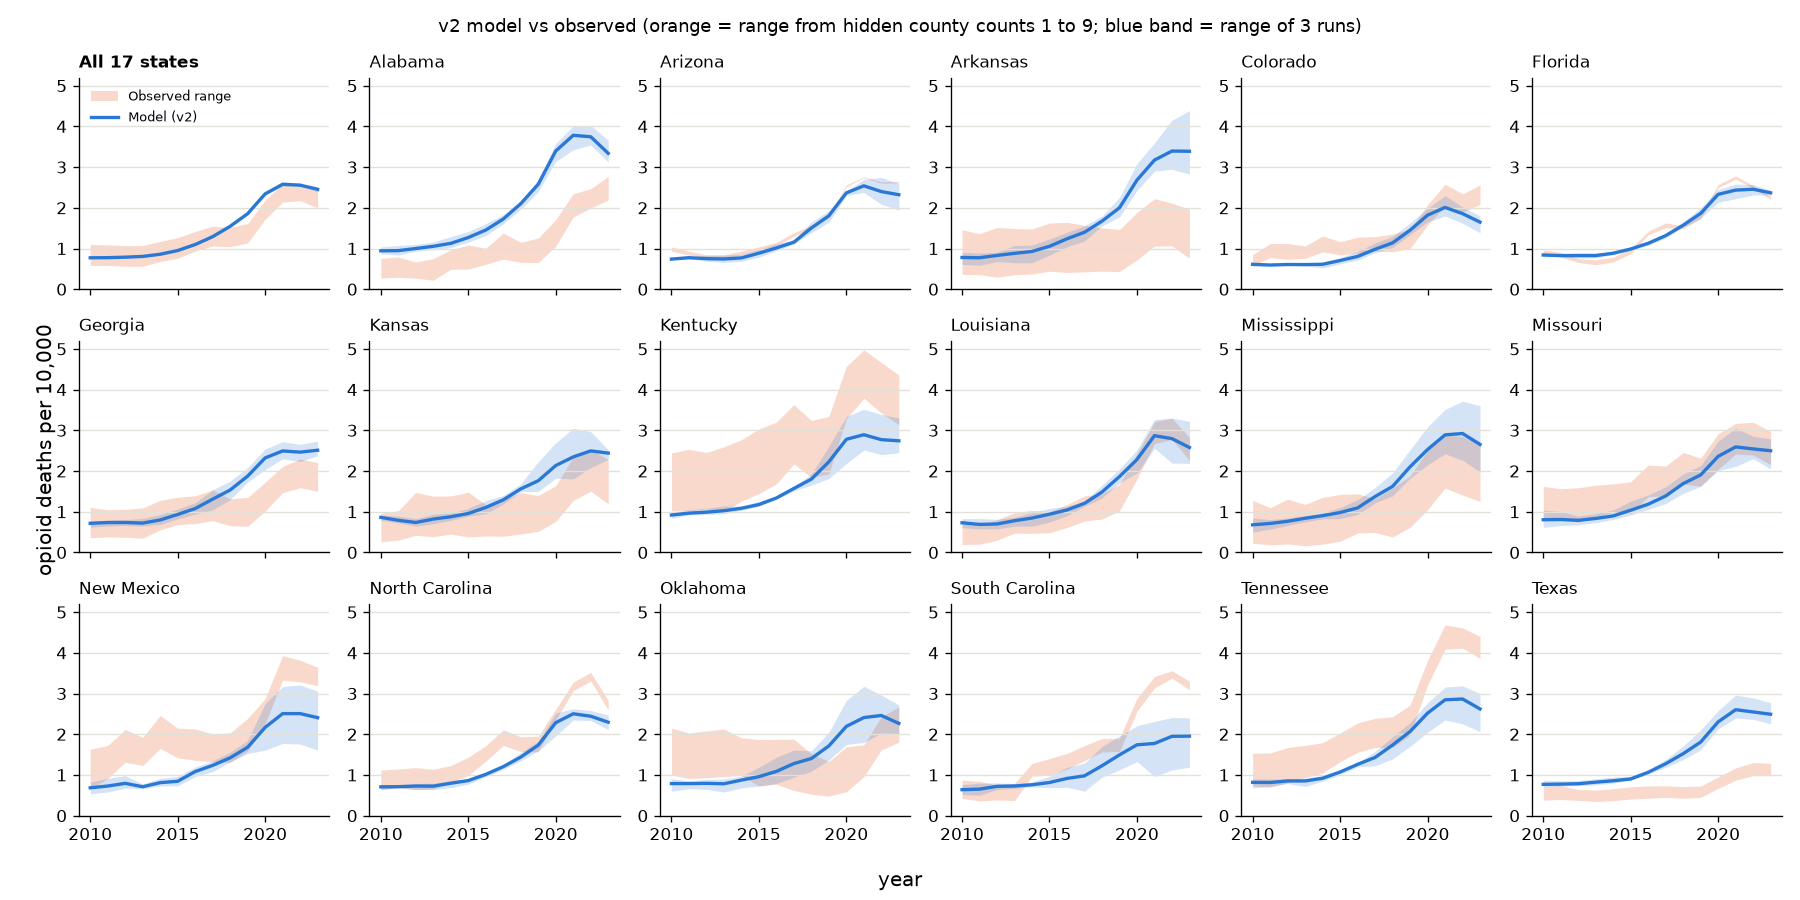
\includegraphics[width=\linewidth]{../../outputs/v2_deaths_by_state.png}
 \column{0.32\textwidth}
 \scriptsize
 \begin{tabular}{@{}lrr@{}}
 \toprule & v1 & v2\\\midrule
 score per state-year & $-70.3$ & $\mathbf{-2.44}$\\
 region, years in range & 11/14 & 10/14\\\bottomrule
 \end{tabular}
 \par\smallskip
 \begin{itemize}\setlength\itemsep{1pt}
  \item Region-wide shape right: flat to 2014, fentanyl rise, 2020 jump, plateau.
  \item COVID jump in \emph{every} state, from each state's own $\psi_s$.
  \item Good: AZ, FL, CO, LA, MO. Too high: TX ($\sim2.5\times$), AL, AR. Too low: KY, TN, SC, NM.
 \end{itemize}
 \end{columns}
\end{frame}

\begin{frame}{Projection to 2060 and a scale test}
 \begin{columns}[T]
 \column{0.52\textwidth}
 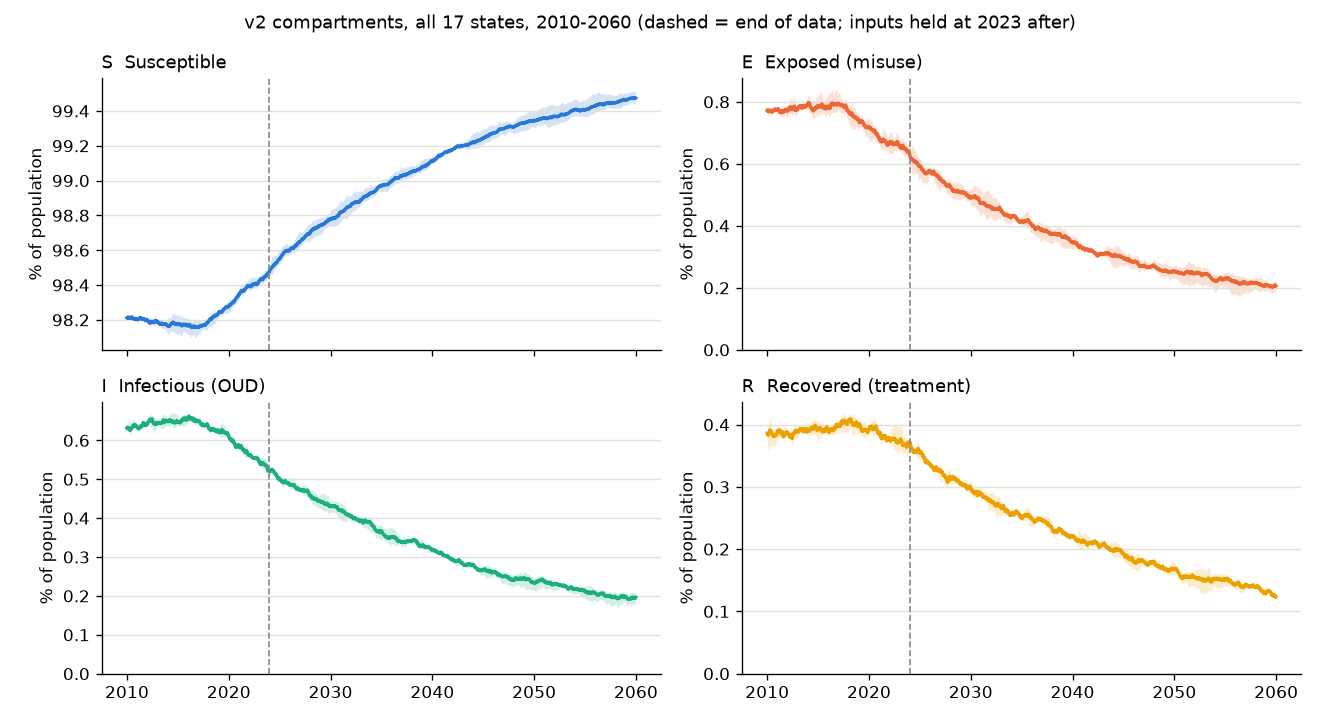
\includegraphics[width=\linewidth]{../../outputs/v2_compartments_2060.png}
 \scriptsize
 \begin{tabular}{@{}lrrrr@{}}
 \toprule \% of population & 2010 & 2023 & 2040 & 2059\\\midrule
 $\Ec$ & .77 & .65 & .34 & .21\\
 $\Ic$ & .63 & .54 & .31 & .19\\
 $\Rc$ & .38 & .37 & .21 & .13\\
 deaths per $10^4$ & .77 & 2.45 & 1.47 & .91\\\bottomrule
 \end{tabular}
 \column{0.45\textwidth}
 \small
 Inputs held at 2023; no state runs away or dies out. Deaths fall more slowly than OUD because $\varphi$ stays at its maximum.
 \par\smallskip
 \begin{block}{$N\times5$ and $h\times2$ (1.5M agents, 30 km)}\scriptsize
 \renewcommand{\arraystretch}{1.15}
 \begin{tabular}{@{}lrr@{}}
 \toprule & 300k, 15 km & 1.5M, 30 km\\\midrule
 region 2021 & 2.58 & 2.54\\
 SD of state rates & .172 & .075\\
 state spread 2021 & 1.77--3.78 & 1.98--3.07\\
 score & $-2.44$ & $-2.23$\\\bottomrule
 \end{tabular}
 \par\smallskip
 SD ratio $0.172/0.075=2.3\approx\sqrt5$: the predicted Monte-Carlo scaling. Caveat: $N$ and $h$ changed together.
 \end{block}
 \end{columns}
\end{frame}

\begin{frame}{Open problems for a mathematical audience}
 \begin{enumerate}\setlength\itemsep{4pt}
  \item \textbf{Identifiability across states.} With literature-sized weights the 17 states look too alike. The missing ingredient is probably \emph{when} fentanyl reached each market, for which we have no data. Is $\varphi_s(t)$ identifiable from state-year totals alone?
  \item \textbf{Mean-field limit.} A proof that the agent system converges to the averaged equations (propagation of chaos) for this interaction kernel and pseudo-count correction is not given here.
  \item \textbf{Stability of the endemic state.} The supply tipping point $\theta_d\approx0.2$ was found numerically; a Jacobian analysis of the coupled $(i,v)$ system is open.
  \item \textbf{Confounding of $N$ and $h$.} A $1.5$M, $15$ km run would separate them.
  \item \textbf{Not modelled:} deaths while in treatment ($\Rc\to\Dc$, $5$--$10\times$ lower), migration, stimulants, naloxone.
 \end{enumerate}
\end{frame}

\begin{frame}{The whole model on one slide}
 \small
 \begin{align*}
  &\textbf{Data}\ x\ \xrightarrow{\ z,\ \operatorname{std}\ }\ \bm\xi\ \xrightarrow{\ s_k\bar w\ }\ F=e^{\bm w\cdot\bm\xi},\qquad a=\tfrac{x^{Rx}}{100},\qquad \psi_s=\tfrac{x^{str}_s}{100}\\
  &\textbf{Market}\quad \dd v_c=[\kappa_v(v^\ast_c-v_c)-D_v((I-W)v)_c]\dd t+\tau_vv_c\dd B_c,\qquad
   \dot\varphi_s=(p_\varphi+p_{cov}\psi_s+q_\varphi\varphi_s)(1-\varphi_s)\\
  &\textbf{Agents}\quad X_i\in\{\Sc,\Ec,\Ic,\Rc\},\quad \lambda_{XY}=\big[\lambda^0_{XY}g_{XY}+\gamma_{XY}\pi^Z_i\big]F_{XY},\quad \pi^X_i=\tfrac{\#_h(X)+k_0x_c}{|B_i|+k_0}\\
  &\textbf{Step}\quad \Pr(\text{leave})=1-e^{-\Lambda\Delta t},\quad \Pr(Y\mid\text{leave})=\lambda_{XY}/\Lambda,\quad \Dc\to\Sc\ \text{in place}\\
  &\textbf{Calibrate (closed form)}\ (\beta^0,\chi)\ \ \text{from}\ (i^\ast,f);\qquad \textbf{match}\ (s_k)\ \text{from}\ \partial\ln m^\ast/\partial\xi^k\\
  &\textbf{Fit (4 numbers)}\ (m_F,p_\varphi,p_{cov},w_{iso})=\arg\max\ \tfrac1{|\mathcal S||\mathcal Y|}\sum\log\Pr\big(\mathrm{NB}(\widehat M_{sy})\in[L_{sy},U_{sy}]\big)
 \end{align*}
 \begin{kept}
  Everything not in the last line is literature, assumption, or a closed-form consequence of a non-death target.
 \end{kept}
\end{frame}

%==================================================================
\appendix
\section{Appendix}
\begin{frame}{Symbol index (1/2)}
 \footnotesize
 \renewcommand{\arraystretch}{1.3}
 \begin{tabularx}{\textwidth}{@{}l X l@{}}
 \toprule Symbol & Meaning & Section\\\midrule
 $\Sc,\Ec,\Ic,\Rc,\Dc$ & susceptible, misuse, OUD, treatment, death (flux) & 1\\
 $s,e,i,r$; $x_c$ & class fractions; county fraction of a class & 1, 4\\
 $x^j,\ z^j,\ \xi^k$ & raw variable; clipped $z$-score; structural index & 2\\
 $w_{\theta k}=s_k\bar w_{\theta k}$ & log-weight of index $k$ on rate $\theta$; scalar times sign-prior & 2\\
 $F_\theta$ & rate modifier $\exp(\bm w_\theta\cdot\bm\xi)$ & 2\\
 $\tau_k$ & elasticity target for index $k$ & 2\\
 $a_c$, $v_c$, $\varphi_s$, $\psi_s$ & prescriptions; illicit supply; fentanyl share; COVID stringency & 3\\
 $\mathcal D_c$, $\bar{\mathcal D}_0$ & local demand; baseline regional demand & 3\\
 $\kappa_v,\ D_v,\ \tau_v,\ \ell,\ \theta_d$ & supply speed, spill-over, volatility, length, demand elasticity & 3\\
 $W_{cc'}$ & row-stochastic proximity weights, $\propto e^{-d_{cc'}/\ell}$ & 3\\
 $p_\varphi,\ q_\varphi,\ p_{cov}$ & Bass innovation, imitation, COVID push & 3\\
 $w_{iso}$ & isolation effect on overdose rate & 3, 5\\
 $N,\ n_c,\ P_c$ & agents, agents in $c$, real population & 4\\
 $h,\ k_0,\ B_i,\ \pi^X_i$ & radius, pseudo-count, neighbour set, local share & 4\\
 \bottomrule
 \end{tabularx}
\end{frame}

\begin{frame}{Symbol index (2/2)}
 \footnotesize
 \renewcommand{\arraystretch}{1.3}
 \begin{tabularx}{\textwidth}{@{}l X l@{}}
 \toprule Symbol & Meaning & Section\\\midrule
 $\lambda_{XY},\ \Lambda_X$ & transition rate; total out-rate & 1, 5\\
 $\beta^0,\ \gamma_{Rx},\ \chi,\ \alpha$ & contact baseline; onset per therapy year; therapy share; $\alpha=\gamma_{Rx}\chi$ & 5\\
 $\sigma^0,\ \epsilon^0$ & $\Ec\to\Ic$, $\Ec\to\Sc$ baselines & 5\\
 $\zeta^0,\ \gamma_p$ & $\Ic\to\Rc$ baseline; peer recovery & 5\\
 $\nu^0$ & $\Ic\to\Sc$ baseline & 5\\
 $\mu_H,\ m_F,\ \kappa=m_F-1$ & overdose hazard without fentanyl; fentanyl multiplier; excess & 5\\
 $\delta^0$ & $\Rc\to\Sc$ baseline & 5\\
 $\rho^0,\ \rho_p$ & relapse: spontaneous, peer & 5\\
 $\vartheta,\ \Pi_i$ & recruiting power of $\Ec$; contagion pressure $\pi^I+\vartheta\pi^E$ & 5\\
 $i^\ast,\ f,\ \bar a$ & calibration targets: prevalence, misuse flux; mean Rx at $t_0$ & 6\\
 $\Rzero,\ T_I,\ p_{RI}$ & reproduction number; time in OUD; relapse probability & 6\\
 $m^\ast$ & long-run deaths per 10{,}000 (mean field) & 2, 6\\
 $\widehat m_c,\ \widehat M_s$ & expected deaths, county, state & 7\\
 $L_{sy},\ U_{sy},\ r,\ \nbc$ & censoring interval; NB size ($50$); NB cdf & 7\\
 \bottomrule
 \end{tabularx}
\end{frame}

\end{document}

